\documentclass[a4paper,12pt]{article}
\usepackage[utf8]{inputenc}
\usepackage{amsmath}
\usepackage{graphicx}
\usepackage{float} 
\usepackage{svg}
\usepackage{hyperref}
\usepackage{minted}  
\usepackage{titlesec}

\setcounter{section}{-1}

\title{You Only Look Once (Yolo)}
\author{BEX Roméo, RIVALDI Tristan, LAMURE Maxence}
\date{24 Septembre 2024}

\begin{document}

\maketitle

\tableofcontents

\newpage

\section{Introduction}

La détection d'objets est une tâche cruciale en vision par ordinateur, utilisée dans des domaines comme la conduite autonome, la surveillance et les systèmes de sécurité. Elle nécessite non seulement la localisation des objets dans une image, mais aussi leur classification, tout en garantissant un temps de traitement rapide pour les applications en temps réel.

L'approche YOLO (You Only Look Once) révolutionne la détection d'objets en traitant cette tâche comme un problème de régression unique, passant directement de l'image complète aux prédictions des boîtes englobantes et des classes d'objets. Cette méthode permet d'atteindre des vitesses élevées, jusqu'à 45 images par seconde, ce qui est idéal pour les systèmes en temps réel. Cependant, YOLO présente certaines limites, notamment dans la précision de la détection des petits objets.

Ce rapport explore l'architecture de YOLO, ses fondements mathématiques, ses performances par rapport aux autres méthodes de détection, ainsi que ses avantages, inconvénients, et applications concrètes.

\section{Système de détection Yolo}

\begin{figure}[H]
    \centering
    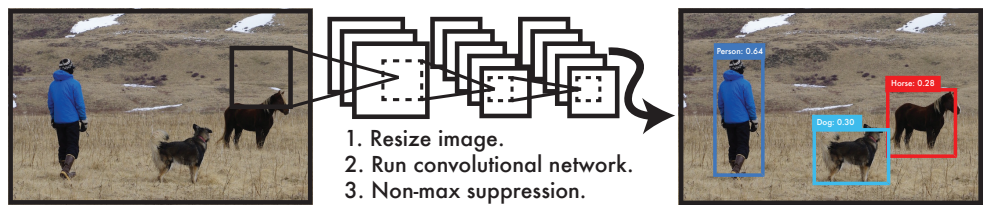
\includegraphics[width=0.9\linewidth]{illustration-yolo.png}
    \caption{Système de détection Yolo}
    \label{fig:enter-label}
\end{figure}

Comme on peut voir ci-dessus, la reconnaissance d'image est divisée en 3 parties qui sont :    
- La première étape consiste à faire un \textbf{redimensionnement} de l'image d'entrée à une taille fixe de 448 × 448 pixels. Cela permet d'uniformiser la taille des images, peu importe leurs dimensions d'origine, ce qui facilite le traitement par le réseau de neurones.

- Ensuite, l'image redimensionnée est passée dans un \textbf{réseau de neurones convolutionnel (CNN)}. Le CNN traite l'image pour extraire des caractéristiques et prédire plusieurs boîtes englobantes (bounding boxes) et les classes d'objets correspondantes. Le réseau prédit simultanément plusieurs objets dans l'image.

- Après que le modèle a généré les prédictions, la dernière étape est \textbf{la suppression non-maximale}. Cette méthode élimine les boîtes englobantes qui se chevauchent et qui représentent le même objet, en ne gardant que la boîte avec le score de confiance le plus élevé. Cela permet d'éviter les multiples détections d'un même objet.


\section{Division de l'image en grille}
YOLO divise l'image d'entrée en une grille de taille $S \times S$. Chaque cellule de la grille est responsable de la prédiction des objets dont le centre tombe dans cette cellule. Pour chaque cellule, le réseau prédit :

\begin{itemize}
    \item $B$ boîtes englobantes (bounding boxes), chaque boîte définie par les coordonnées du centre $(x, y)$, la largeur $w$ et la hauteur $h$.
    \item Un score de confiance qui reflète la précision de la boîte englobante et la probabilité qu'un objet soit présent dans cette boîte.
    \item $C$ probabilités de classe, où $C$ est le nombre de classes d'objets prédictibles.
\end{itemize}

Ainsi, la sortie du modèle est un tenseur de dimension :
\[
S \times S \times (B \times 5 + C)
\]
où $B \times 5$ correspond aux prédictions pour les boîtes (5 valeurs par boîte : $x$, $y$, $w$, $h$ et la confiance) et $C$ est le nombre de classes.

\section{Prédiction des boîtes englobantes}
Chaque boîte englobante est prédite avec 5 paramètres :
\begin{itemize}
    \item $(x, y)$ : Les coordonnées du centre de la boîte par rapport aux limites de la cellule.
    \item $w$ et $h$ : La largeur et la hauteur de la boîte, relatives à la taille de l'image.
    \item \textbf{Confiance} : Définie par le produit suivant :
    \[
    \text{Confiance} = \text{Pr}(\text{Object}) \times \text{IoU}_{\text{pred, truth}}
    \]
    où $\text{IoU}_{\text{pred, truth}}$ (Intersection over Union) mesure le chevauchement entre la boîte prédite et la boîte réelle (ground truth).
\end{itemize}

La confiance représente à la fois la probabilité qu'un objet soit présent dans la boîte et l'ajustement de la boîte par rapport à l'objet réel.

\section{Fonction de perte}
La fonction de perte de YOLO est composée de plusieurs parties, correspondant à différents types d'erreurs :

\subsection{Perte de localisation}
La \textbf{perte de localisation} évalue la précision des coordonnées prédite pour les boîtes englobantes. Elle compare les prédictions $(x, y, w, h)$ aux valeurs réelles (ground truth).

\[
\text{Loss}_{\text{loc}} = \lambda_{\text{coord}} \sum_{i=0}^{S^2} \sum_{j=0}^{B} \mathbf{1}_{\text{obj}}^{ij} \left[ (x_i - \hat{x}_i)^2 + (y_i - \hat{y}_i)^2 + \left( \sqrt{w_i} - \sqrt{\hat{w}_i} \right)^2 + \left( \sqrt{h_i} - \sqrt{\hat{h}_i} \right)^2 \right]
\]
où :
\begin{itemize}
    \item $(x_i, y_i)$ et $(\hat{x}_i, \hat{y}_i)$ sont les coordonnées du centre prédites et réelles.
    \item $w_i$, $h_i$ et $\hat{w}_i$, $\hat{h}_i$ sont les largeurs et hauteurs prédites et réelles.
    \item $\mathbf{1}_{\text{obj}}^{ij}$ est un indicateur qui vaut 1 si l'objet est présent dans la cellule $i$ pour la boîte $j$, sinon 0.
    \item $\lambda_{\text{coord}}$ est un facteur de pondération qui donne plus d'importance à la précision de la localisation.
\end{itemize}

\subsection{Perte de confiance}
La \textbf{perte de confiance} évalue l'erreur entre la confiance prédite et la réalité. Elle se divise en deux parties :
\begin{itemize}
    \item Lorsque l'objet est présent :
    \[
    \text{Loss}_{\text{conf\_obj}} = \sum_{i=0}^{S^2} \sum_{j=0}^{B} \mathbf{1}_{\text{obj}}^{ij} (C_i - \hat{C}_i)^2
    \]
    \item Lorsque l'objet n'est pas présent :
    \[
    \text{Loss}_{\text{conf\_noobj}} = \lambda_{\text{noobj}} \sum_{i=0}^{S^2} \sum_{j=0}^{B} \mathbf{1}_{\text{noobj}}^{ij} (C_i - \hat{C}_i)^2
    \]
    où $\lambda_{\text{noobj}}$ est un facteur de pondération pour les boîtes sans objets.
\end{itemize}

\subsection{Perte de classification}
La \textbf{perte de classification} compare les probabilités de classe prédites aux classes réelles :
\[
\text{Loss}_{\text{class}} = \sum_{i=0}^{S^2} \mathbf{1}_{\text{obj}}^{i} \sum_{c \in \text{classes}} (p_i(c) - \hat{p}_i(c))^2
\]
où $p_i(c)$ est la probabilité prédite pour la classe $c$ dans la cellule $i$, et $\hat{p}_i(c)$ est la probabilité réelle.

\subsection{Fonction de perte totale}
La fonction de perte totale est donnée par la somme des trois composantes précédentes :
\[
\text{Loss}_{\text{total}} = \text{Loss}_{\text{loc}} + \text{Loss}_{\text{conf\_obj}} + \text{Loss}_{\text{conf\_noobj}} + \text{Loss}_{\text{class}}
\]

\section{Intersection over Union (IoU)}
L'IoU est une mesure clé utilisée pour évaluer la qualité des boîtes englobantes prédite. Il est défini comme le rapport entre l'aire de l'intersection et l'aire de l'union des deux boîtes :
\[
\text{IoU}(B_{\text{pred}}, B_{\text{truth}}) = \frac{\text{Aire}(B_{\text{pred}} \cap B_{\text{truth}})}{\text{Aire}(B_{\text{pred}} \cup B_{\text{truth}})}
\]
Si l'IoU est supérieur à un certain seuil (généralement 0.5), la boîte prédite est considérée comme correcte.

\section{Conclusion}
L'algorithme YOLO propose une approche simple mais puissante pour la détection d'objets en temps réel. En reformulant la détection comme un problème de régression, YOLO permet de prédire simultanément plusieurs boîtes et classes dans une image, le tout en une seule passe à travers le réseau. La fonction de perte soigneusement conçue optimise à la fois la localisation des objets, la confiance des prédictions, et la classification.

\end{document}
 